%%%%%%%%%%%%%%%%%%%%%%%%%%%%%%%%%%%%%%%%%%%%%%%%%%%%%%%%%%%%%%%%%%%%%%%%%%%%%%
\section{Simulation of the $\pi+ \to e^+ \nu $ signal }

{\red Briefly Describe the multistage simulation - standard Mu2e scheme
  \begin{itemize}
  \item
    first: simulation of pion beam
  \item
    then - simulation of the $\pi^+ \to e^+ \nu$ decays in the detector
  \end{itemize}
}
%%%%%%%%%%%%%%%%%%%%%%%%%%%%%%%%%%%%%%%%%%%%%%%%%%%%%%%%%%%%%%%%%%%%%%%%%%%%%% 
\subsection {Pion lifetime: validation}

Weighting events with the pion lifetime - validation plot here

\begin{figure}[H]
  \begin{tikzpicture}
    \node[anchor=south west,inner sep=0] at (0,0.) {
      % \node[shift={(0 cm,0.cm)},inner sep=0,rotate={90}] at (0,0) {}
      \makebox[\textwidth][c] {
        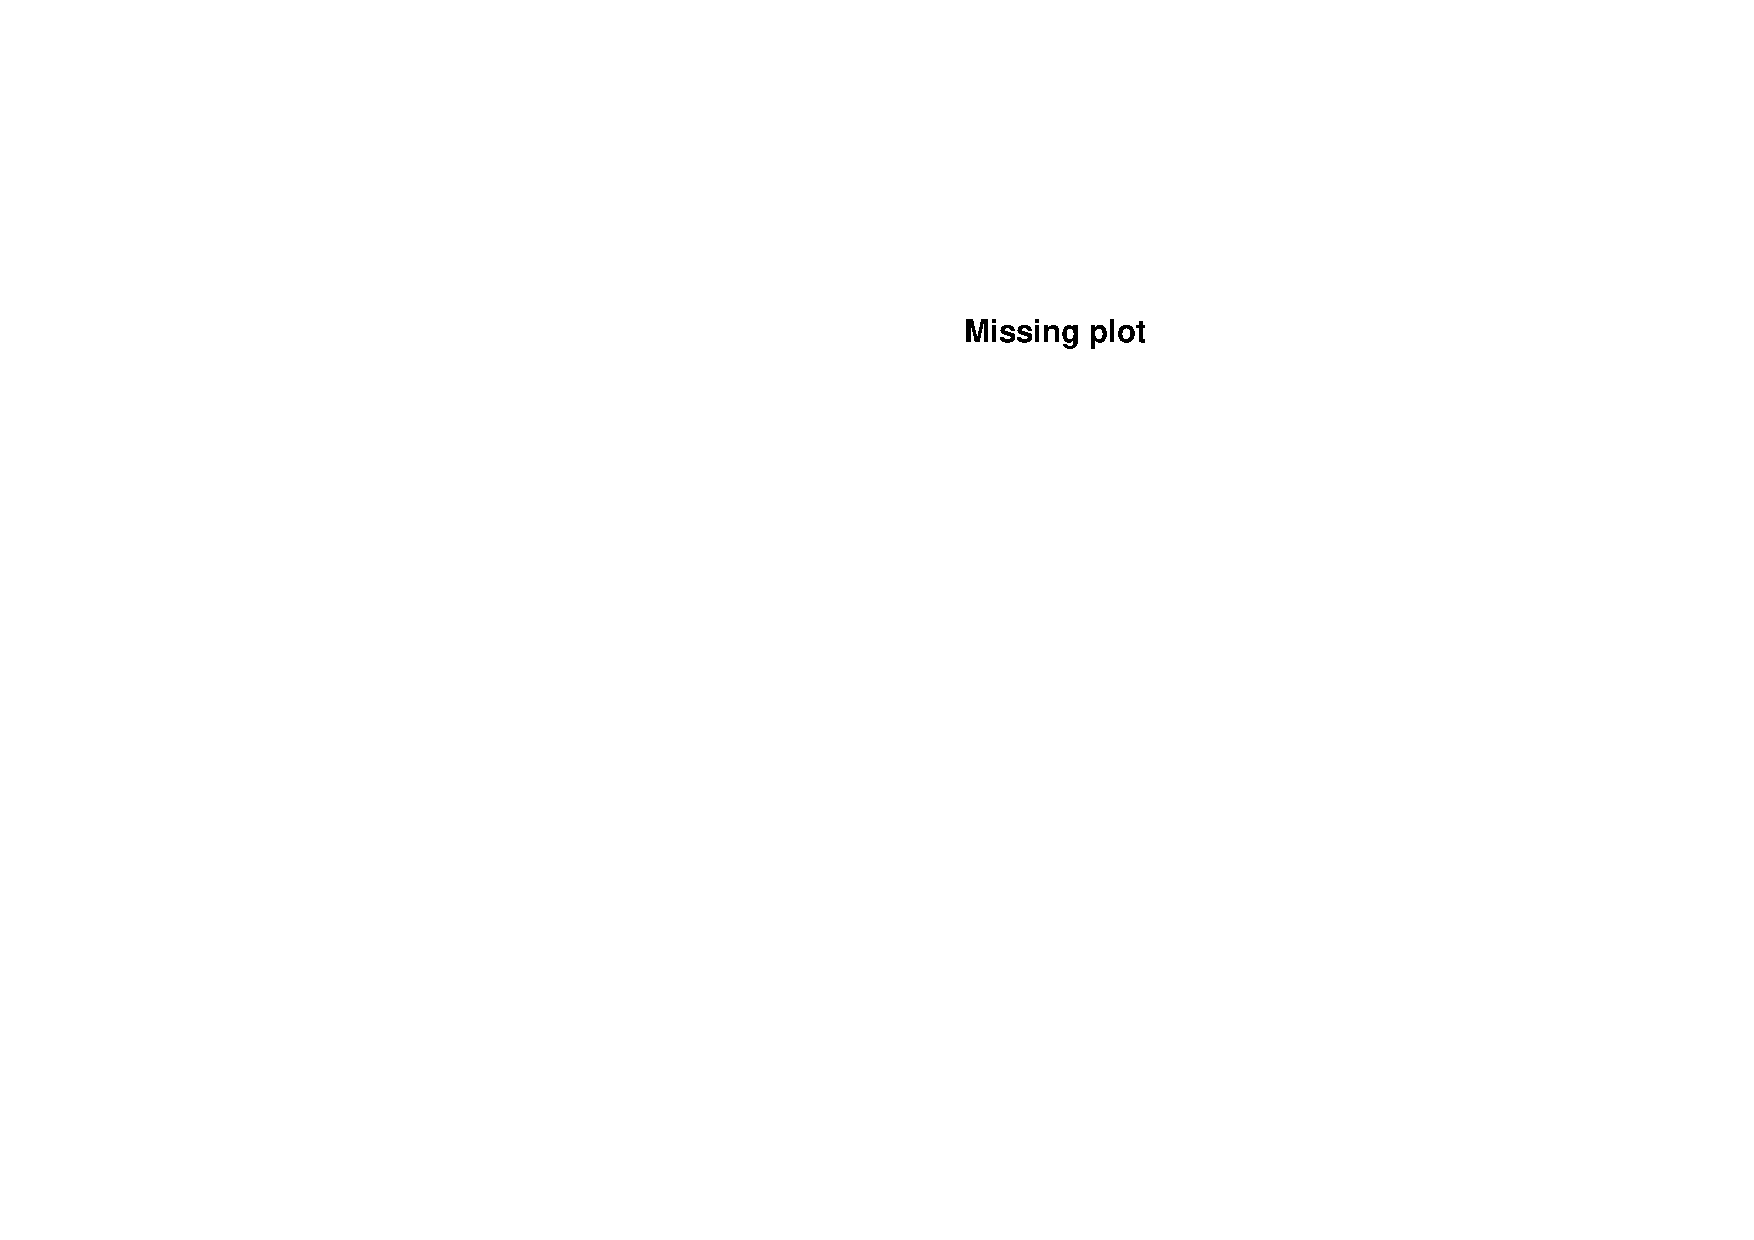
\includegraphics[width=1.0\textwidth]{pdf/missing_plot}
      }
    };
    \node [text width=8cm, scale=1.0] at (14.5,0.5) {$\mu_B$, expected background mean};
    \node [text width=8cm, scale=1.0, rotate={90}] at (1.5,7.5) { $S_{D}$, ``discovery'' signal strength  };
  \end{tikzpicture}
  \caption{
    \label{fig:pion_lifetime}
  }
\end{figure}

To increase statistics, the pion beam simulation had the charged pion decays turned off.
The survival probability of stopped $\pi^+$'s was stored and used in the analysis
as the event weight.

%%%%%%%%%%%%%%%%%%%%%%%%%%%%%%%%%%%%%%%%%%%%%%%%%%%%%%%%%%%%%%%%%%%%%%%%%%%%%% 
\subsection{Comparison to the BU analysis}

{\red 
\begin{itemize}
\item 
  Compare the signal yield/POT  - should be stable enough.
\item
  BU number : (after all cuts - mu2e-5391 , what are they?): $2.3 x 10^{-12}$ / POT
\end{itemize}
}

